\documentclass[usepdftitle=false]{beamer}
\usetheme{Berkeley}

% introducido por mi 
\usepackage{amsmath,amsfonts,amssymb} % ecuaciones
\usepackage{siunitx}
\usepackage{fancyhdr} % headers y footers
\usepackage{esint} % integrales cerradas
\usepackage{bbold} % para meter matriz identidad
\usepackage{graphicx} % estos dos para una figura
\usepackage[font=tiny]{caption}
\usepackage{pdfpages} % para incluir declaracion IA
\usepackage{float}
\usepackage{url}
\usepackage[export]{adjustbox}
\usepackage[bottom]{footmisc}
\usepackage{hyperref} % to add video
%\usepackage{footbib}

\newcommand{\xd}{\dot{x}}
\newcommand{\xdd}{\ddot{x}}
\newcommand{\yd}{\dot{y}}
\newcommand{\ydd}{\ddot{y}}
\newcommand{\bigO}{\mathcal{O}}

\title[]{On wave propagation in altermagnets}
\author{Victor Garcia Cervantes}
\institute{University of Amsterdam}
\date{2025-2026}
\setbeamertemplate{footline}[frame number]
\titlegraphic{
\includegraphics[height=2cm]{Uva_logo.png}}

\begin{document}
\frame{\titlepage}

\begin{frame}{Contents}
\tableofcontents
\end{frame}

\begin{frame}{Supervisors}
    \begin{columns}[t]
\column{.45\textwidth}
\centering
\begin{figure}
    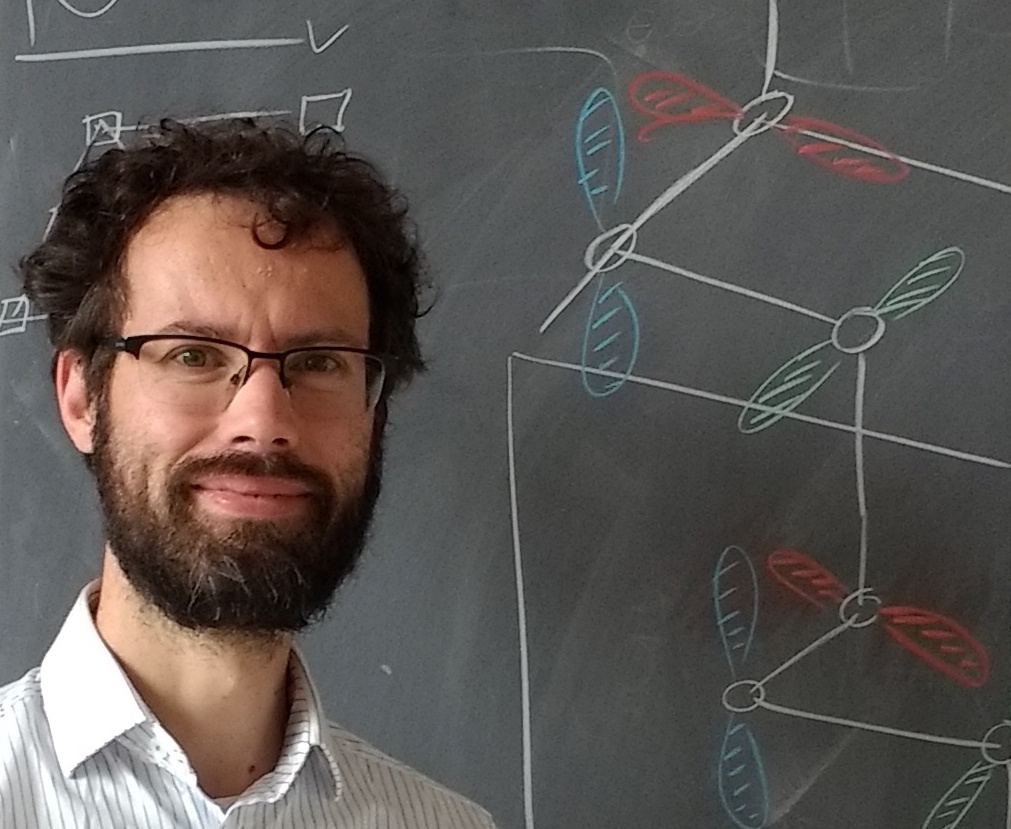
\includegraphics[height=3cm]{Jasper1.jpg}%\caption{Prof. Jasper van Wezel}
\end{figure}
\begin{figure}
    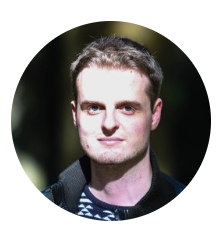
\includegraphics[height=3cm]{viktor.png}%\caption{Dr. Viktor Könye}
\end{figure}
\column{.45\textwidth}
\centering
\begin{figure}
    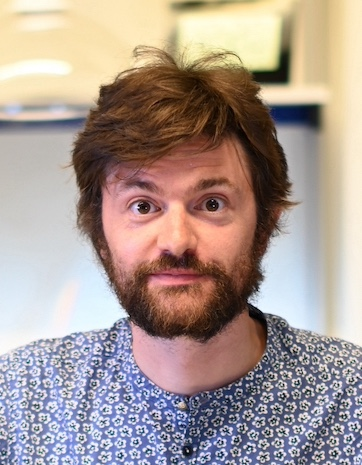
\includegraphics[height=3cm]{corentin.jpg}%\caption{Dr. Corentin Coulais}
\end{figure}
\begin{figure}
    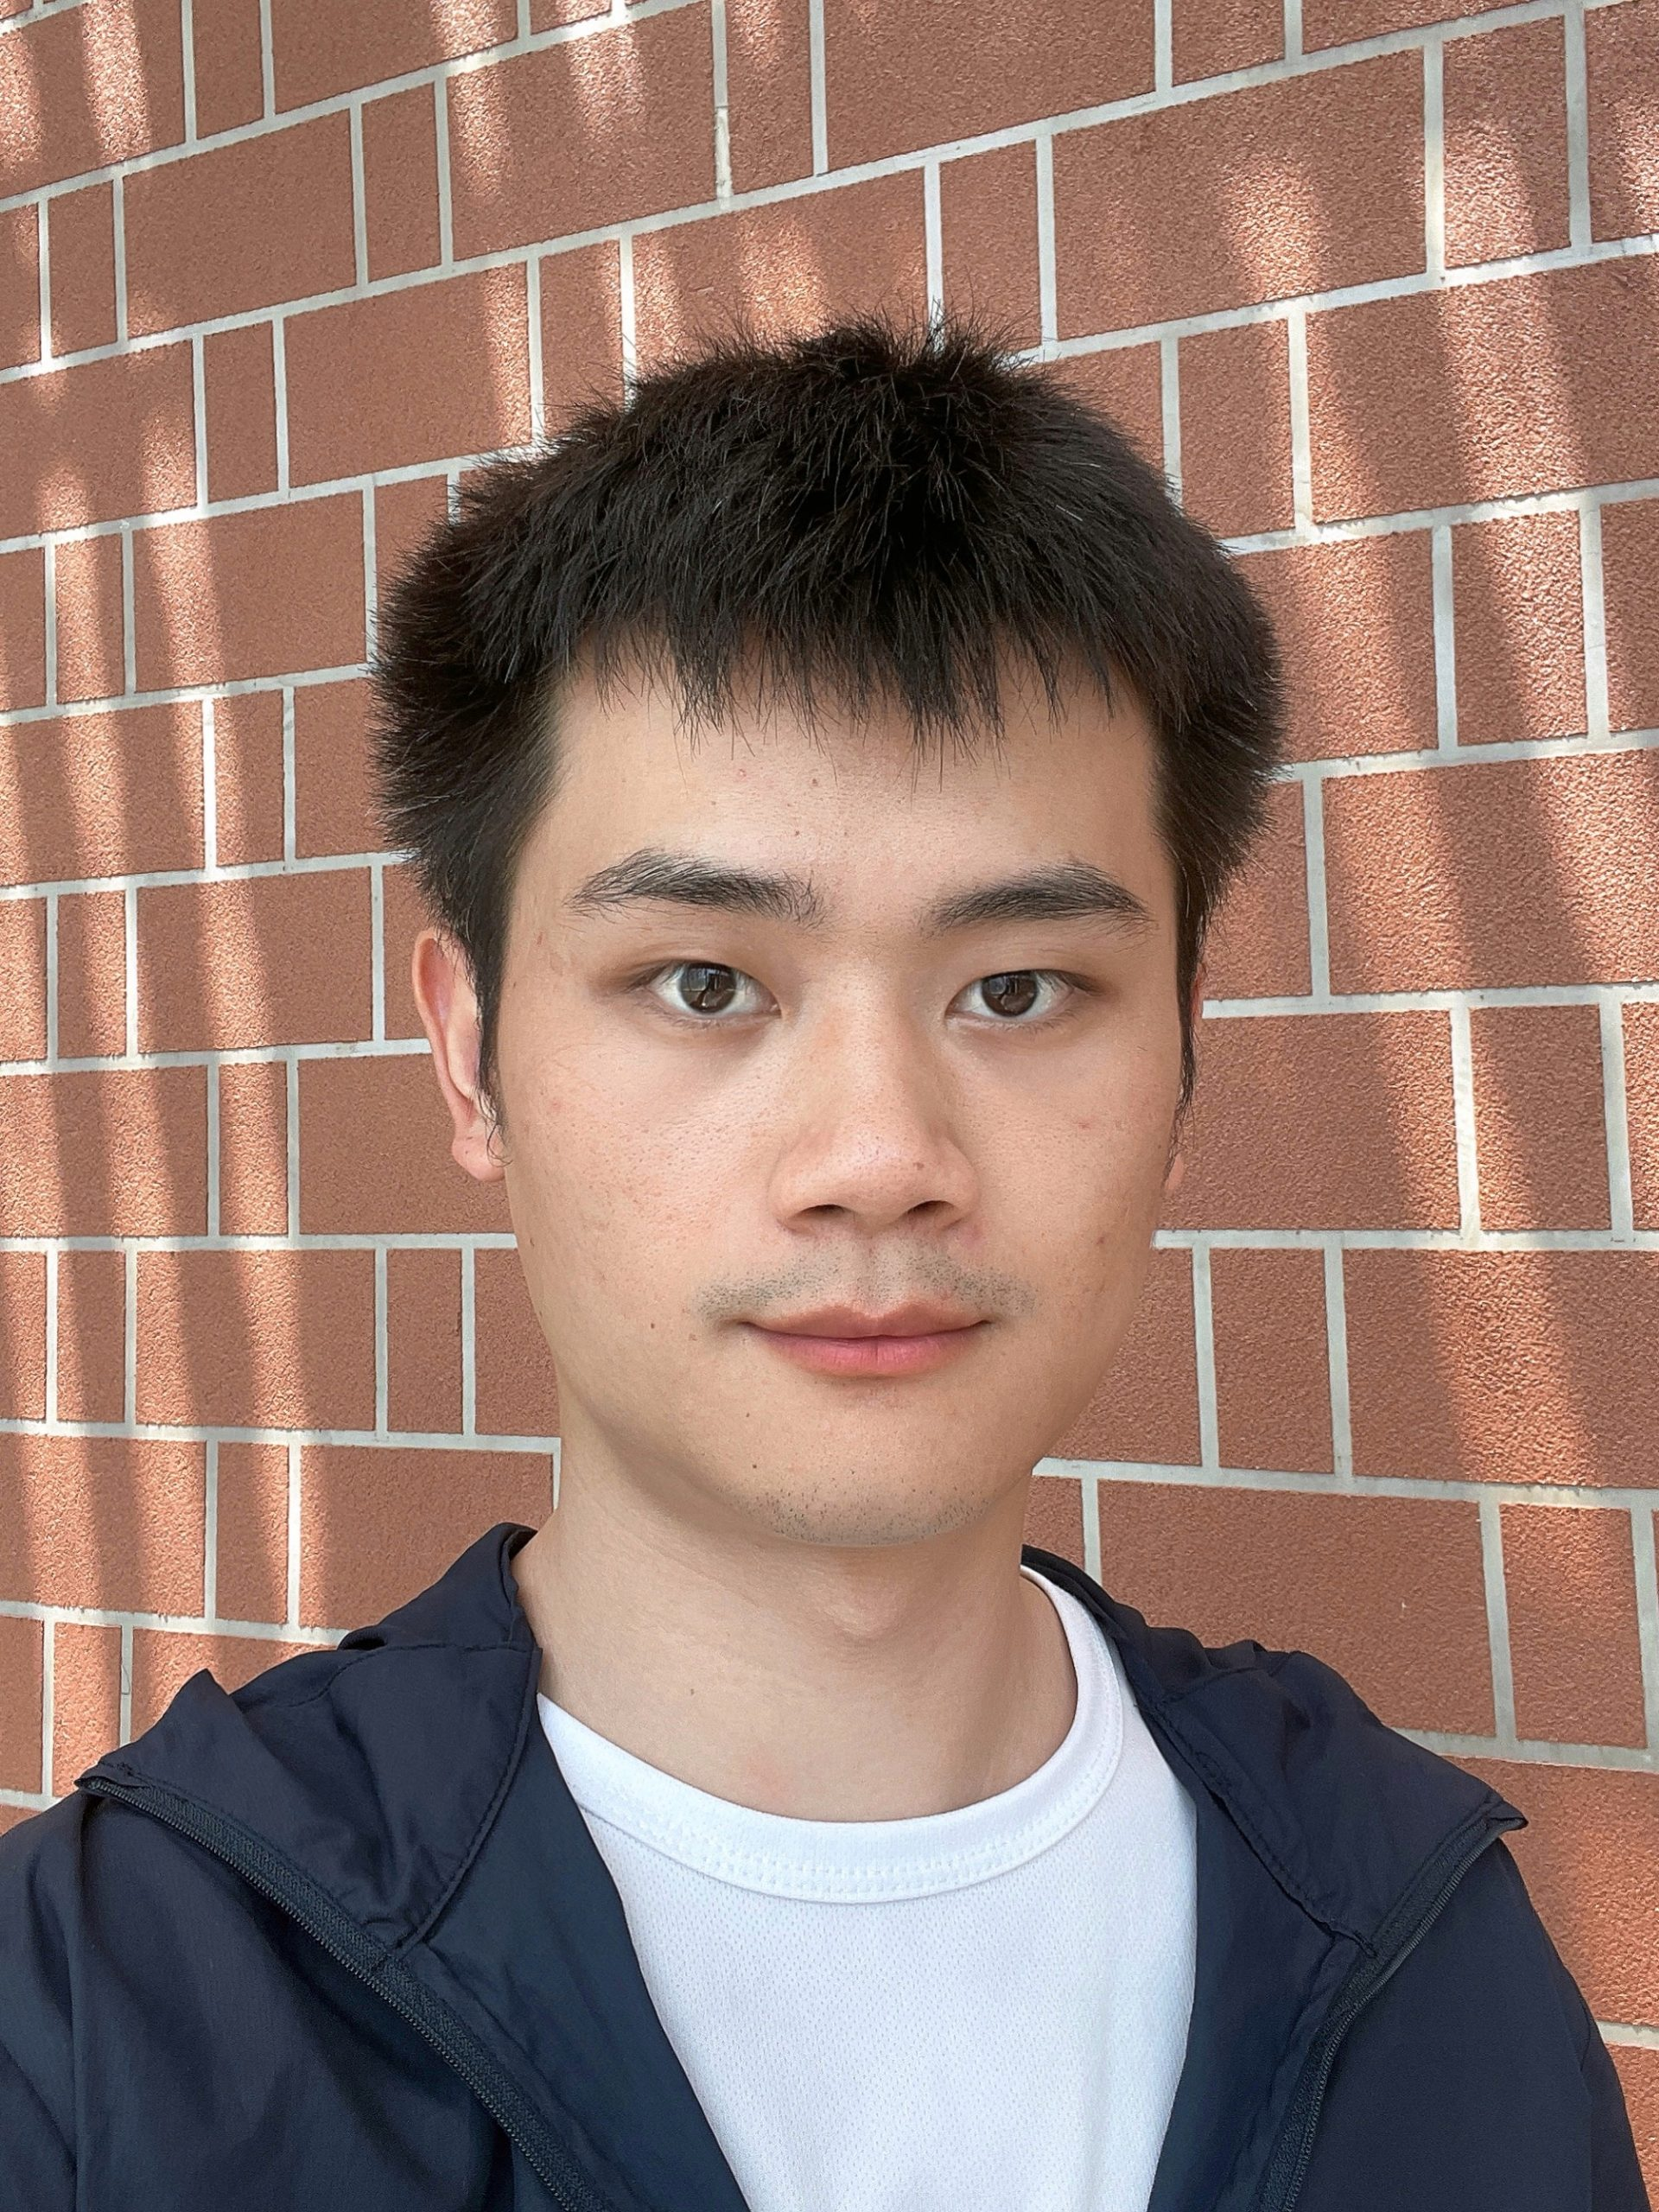
\includegraphics[height=3cm]{yuan.jpeg}%\caption{Dr. Yuan Zhou}
\end{figure}
\end{columns}
\end{frame}

\begin{frame}{Simulation Results}
    Click the image below to play the simulation video:
    
    \vspace{0.5cm}
    \centering
    % "run:" tells the PDF viewer to execute/open the file externally
    \href{run:MicrosoftTeams-video.mp4}{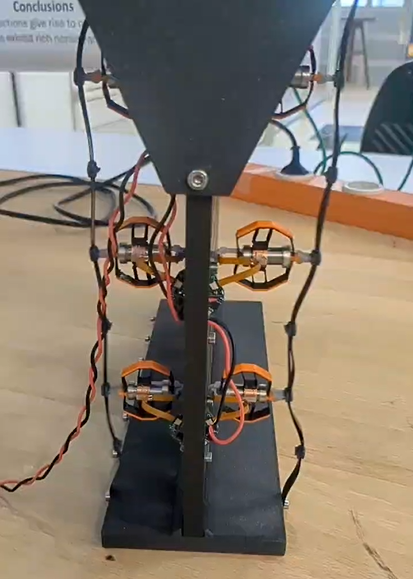
\includegraphics[width=0.3\textwidth]{first_frame_video_exp_setup_slowmo.PNG}}
\end{frame}

\section{Wave propagation}

\begin{frame}{Motivation}
    \begin{alertblock}{What is the project about?}
        Altermagnetic symmetry/Lieb lattice + non-hermiticity/non-reciprocity, in classical analogues
    \end{alertblock}
    \begin{block}{Underlying idea}
        Guide wave signals in solids
    \end{block}
    \pause 
    \vfill
    One can use different excitations: electrons, photons, phonons, etc.
    \pause
    \vfill
    \begin{enumerate}
        \item Anisotropic/directional    
        \item Robust  $\longrightarrow$ topologically protected 
        \item Spin-momentum locking
    \end{enumerate}
\end{frame}

\begin{frame}{Examples}
    Example 1: quantum spin Hall effect
    \begin{figure}
        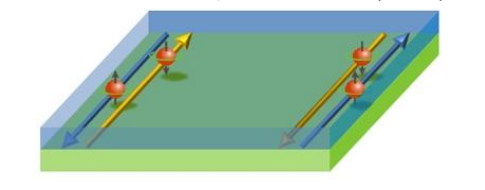
\includegraphics[width = 0.4\textwidth]{qshe_diagram.png}
        \caption{Irene Aguilera Topological materials course}
    \end{figure} \pause 
    Example 2: 2D array of pendula
    \begin{figure}
        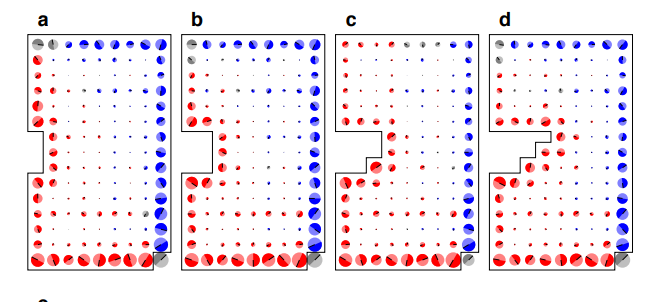
\includegraphics[width = 0.5\textwidth]{huber_pendula_diagram.png}
        \caption{\cite{Huber}}
    \end{figure}
\end{frame}


\section{Altermagnets}

\begin{frame}[allowframebreaks]{What are altermagnets? A different phase of matter}
    \begin{figure}
        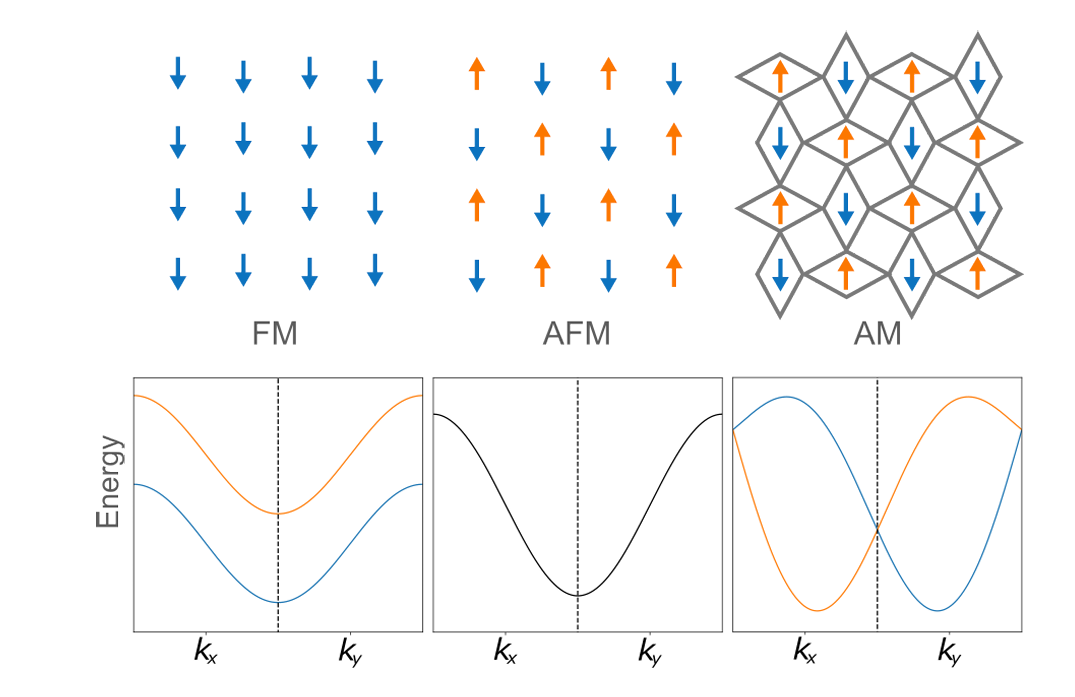
\includegraphics[height=0.8\textheight]{altermagnetism.png}
        \caption{\cite{visser2023}}
    \end{figure} 
    %Kramer's theorem: TRS + half-integer spin $\Longrightarrow$ degenerate energies
    \framebreak
    \begin{enumerate}
        \item Symmetry: Rotation+TR  denoted by $C_4\mathcal{T} $
        \item Zero magnetization  
        \item Spin-split bands
        \item $C_4\mathcal{T} \Longrightarrow N_\uparrow = N_\downarrow$
    \end{enumerate} 
    % include table comparing FM, AFM, AM
    \begin{figure}
        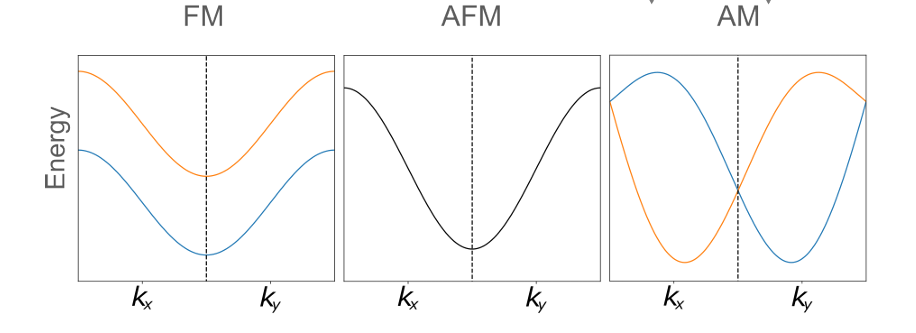
\includegraphics[width=\textwidth]{bands_altermagnet.png}
        \caption{\cite{visser2023}}
    \end{figure}
\end{frame}

\begin{frame}{Lieb lattice as a model altermagnet}
    \begin{figure}
        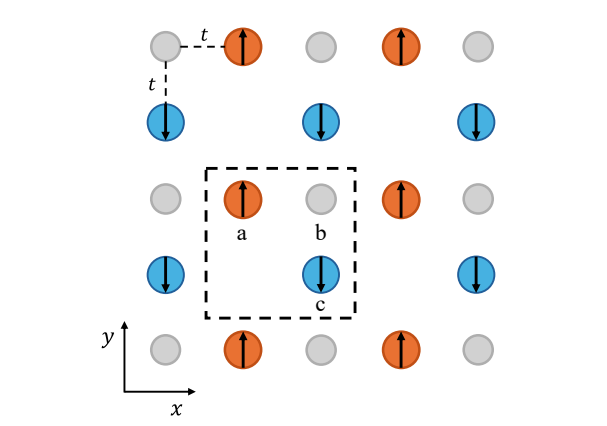
\includegraphics[width = 0.6\textwidth]{Lieb_lattice.png}
        \caption{\cite{visser2023}}
    \end{figure} 
    It has hyperbolic bands:
    \begin{figure}
        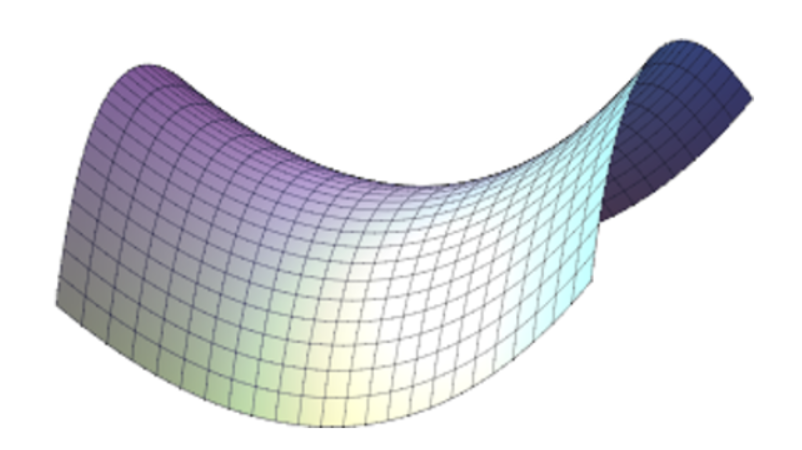
\includegraphics[width = 0.3\textwidth]{hyperbolic_paraboloid.png}
        \caption{Wikipedia}
    \end{figure}
\end{frame}

\begin{frame}{Properties of altermagnets}
    \begin{enumerate}
        \item Anisotropic: control wave propagation direction  \vfill
        \item Spin-momentum locking: different spins propagate in different directions  \vfill
        \item Piezomagnetism: magnetic moment is induced by strain 
        %\item Anomalous Hall effect 
    \end{enumerate}
    \vfill
    Useful in spintronics, spin-splitters, ultrafast photomagnetism, thermoelectrics ...
\end{frame}

\begin{frame}{Generalization of alter symmetry}
    %The lattice symmetry can be generalised to other systems outside of magnetism. \\ \vspace{5mm}
    \begin{alertblock}{Generalization $C_4\mathcal{T} $ symmetry}
        spin $\longrightarrow$ 2-state variable
    \end{alertblock}
    \vfill
    Some examples are:
    \begin{itemize}
        \item Photon polarization $\longrightarrow$ photonic altermagnet  %\tiny{\cite{kim2025photonicaltermagnets}}
        \item Electric dipole $\longrightarrow$ alterelectric  %\tiny{\cite{visser2023}}
        \item Pendula chirality $\longrightarrow$ mechanical altermagnet (metamaterial)
    \end{itemize}
    \begin{figure}
        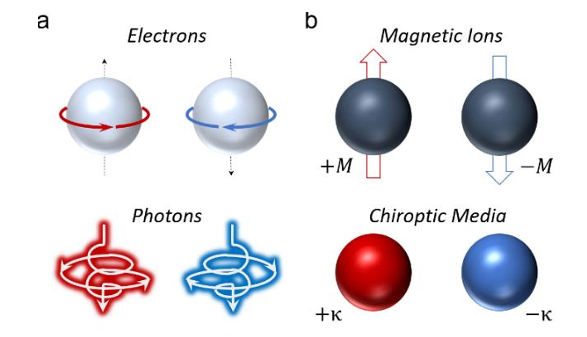
\includegraphics[width = 0.5\textwidth]{photonic_AM.png}
        \caption{\cite{kim2025photonicaltermagnets}}
    \end{figure}
\end{frame}

% \begin{frame}[allowframebreaks]{Metamaterials}
%     Example 1: piezoelectricity
%     \begin{itemize}
%         \item Onsager relations: \begin{align*}
% \varepsilon_{ij} &= S^E_{ijkl}\sigma_{kl} + d_{ijk}E_k, \\
% D_i &= d_{ijk}\sigma_{jk} + \kappa^\sigma_{ik}E_k,
% \end{align*}
%         \item Restrictions due to crystal symmetry: \begin{align*}
% \begin{bmatrix}
% d_{ij} \\
% \end{bmatrix}^T = 
% \begin{bmatrix}
% 0 & 0 & 0 & d_{15} & 0 \\
% 0 & 0 & 0 & d_{24} & 0 \\
% d_{31} & d_{32} & d_{33} & 0 & 0
% \end{bmatrix}^T \quad (j = 1, 2, 3, 4, 5, 6)
% \end{align*} 
%         \item Enhancement due to complex structures  
%         \item Properties given by its structure, not by its parts  
%     \end{itemize}
%     \framebreak
%     Example 2: negative refractive index
%     \begin{figure}
%             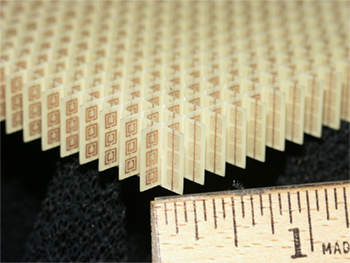
\includegraphics[width = 0.4\textwidth]{Split-ring_resonator_array_10K_sq_nm.jpg}
%         \end{figure}
% \end{frame}

\section{Non-hermiticity}

\begin{frame}[allowframebreaks]{Non-hermiticity}
    \begin{itemize}
        \item Motivation: gain/loss for pendula chirality, non-reciprocal hopping 
        \item In hermitian systems: PBC bulk $\longrightarrow$ OBC edge states
        \item In non-hermitian systems: extreme sensitivity to boundaries 
        \item Spectrum becomes complex
         \begin{figure}
            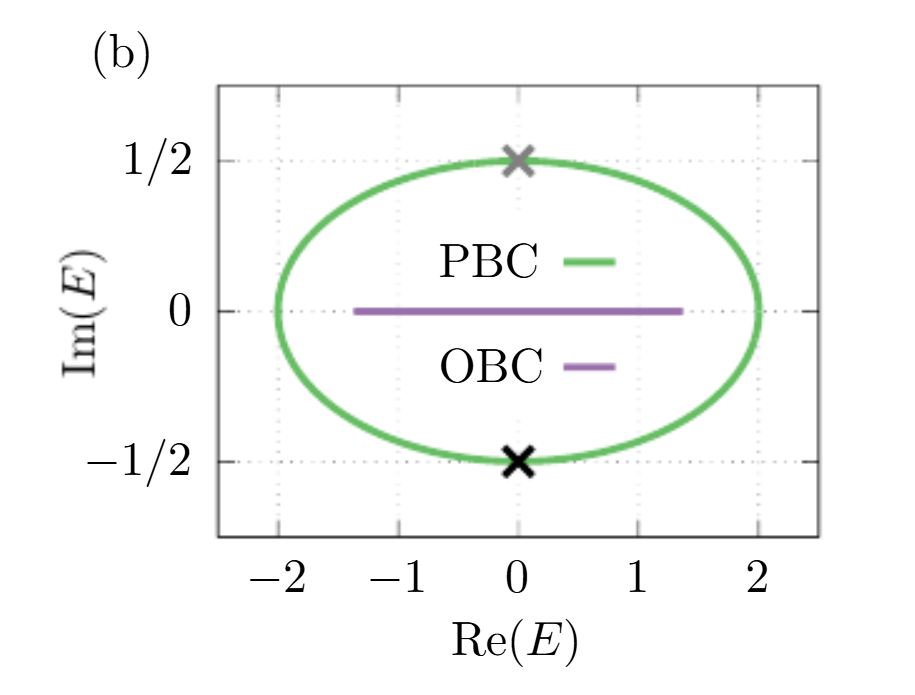
\includegraphics[width = 0.4\textwidth]{hatano-nelson_spectrum.png}
            \caption{\cite{Gohsrich_2025}}
        \end{figure}
        \item \textbf{New} non-hermitian skin effect: eigenstates localize at boundary 
        \item Example: Hatano-Nelson model  
        \begin{align*}
\hat{H}_{\rm HN} = \sum_j \left[ t_Rc_{j+1}^{\dagger} c_j + t_Lc_j^{\dagger} c_{j+1} \right]
\end{align*}
    \end{itemize}
\end{frame}

% \begin{frame}{Non-reciprocity}
%         \begin{minipage}[t]{0.65\textwidth}
%         \begin{itemize}
%             \item Meaning: asymmetric interaction 
%             \item Example: diode
%             \item Motivation: breaks inversion symmetry $\longrightarrow$ directional waves  
%             %\item Response differs when transmitter/receiver swapped \pause
%             %\item Breaks Newton's third law (classical level) \pause
%             \item $\begin{pmatrix}
%             F_1 \\ 
%             F_2
%             \end{pmatrix}
%             =
%             \begin{pmatrix}
%             k & -k^o \\ 
%             +k^o & k
%             \end{pmatrix}
%             \begin{pmatrix}
%             \Delta_1 \\ 
%             \Delta_2
%             \end{pmatrix}$ \pause 
%             \item Non-reciprocal units 
%             %\item Leads to pendula chirality
%         \end{itemize}
%     \end{minipage}%
%     \hfill
%     \begin{minipage}[t]{0.3\textwidth}
%         \vspace{0.5cm}
%         \raggedleft
%         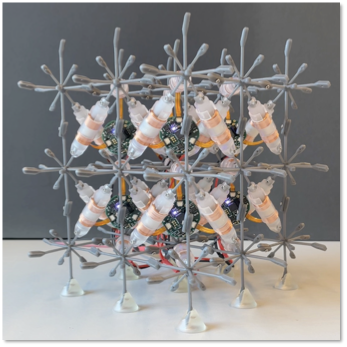
\includegraphics[width=\linewidth]{Yuan_cube_clear.png}
%         %\caption{}
%     \end{minipage}
% \end{frame}

\begin{frame}[allowframebreaks]{Non-reciprocity}
        \begin{itemize}
            \item Meaning: asymmetric interaction 
            \item Example: diode
            \item Motivation: breaks inversion symmetry $\longrightarrow$ directional waves  
            %\item Response differs when transmitter/receiver swapped \pause
            %\item Breaks Newton's third law (classical level) \pause
            \item $\begin{pmatrix}
            F_1 \\ 
            F_2
            \end{pmatrix}
            =
            \begin{pmatrix}
            k & -k^o \\ 
            +k^o & k
            \end{pmatrix}
            \begin{pmatrix}
            \Delta_1 \\ 
            \Delta_2
            \end{pmatrix}$ \pause 
        \begin{figure}
            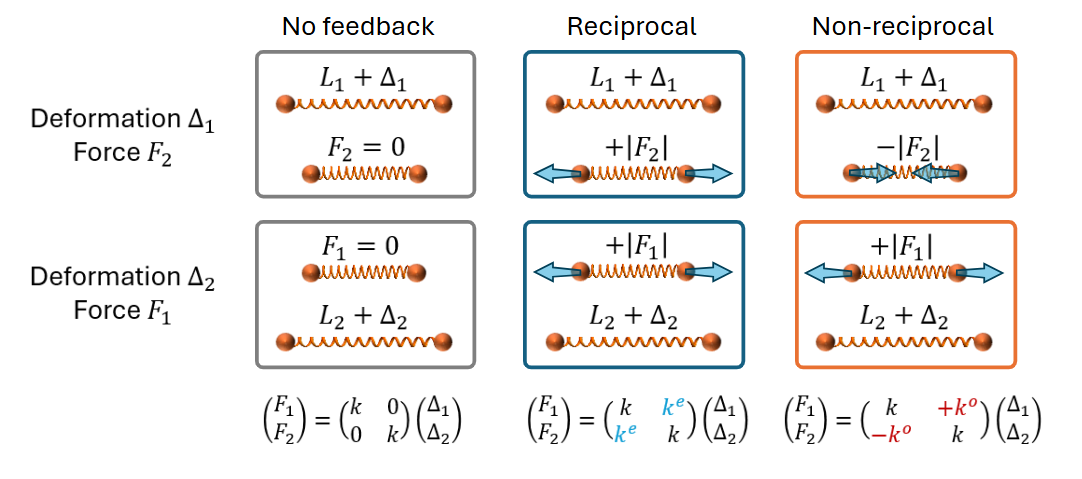
\includegraphics[width=0.8\textwidth]{non_reciprocal_spring_actuators.png}
            \caption{Non-reciprocal actuators}
        \end{figure}
        \framebreak 
        \item Non-reciprocal units 
            %\item Leads to pendula chirality
        \end{itemize}
        \begin{figure}
            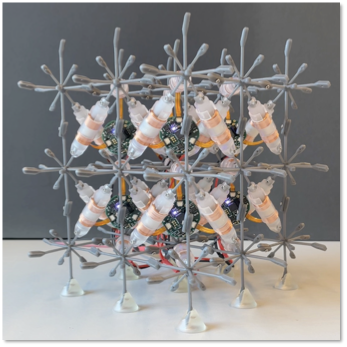
\includegraphics[width=0.5\linewidth]{Yuan_cube_clear.png}
            \caption{3d cube}
        \end{figure}
        
\end{frame}

\section{Getting to the point}

\begin{frame}{In practice}
    \begin{alertblock}{What is the project about?}
        Altermagnetic symmetry/Lieb lattice + non-hermiticity/non-reciprocity, in classical analogues
    \end{alertblock} \pause 
    The procedure has been:  
    \begin{enumerate}
        \item Choose a classical model   
        \item Write equations of motion   
        \item Map to quantum system (using mulitple scale expansion) 
        \item Analyze spectrum and eigenstates \pause 
    \end{enumerate}
    \vfill
    The idea is to apply them to increasingly more complex models.
    \vfill
    \begin{block}{Experimentally}
        Build a Lieb lattice of non-reciprocal pendula and compare with theoretical predictions
    \end{block}
\end{frame}

\begin{frame}[noframenumbering, allowframebreaks]{Multiple scale expansion: the map to quantum system}
    Technique useful for solving nonlinear ODEs with different timescales \\
    \vspace{0.5cm}
    Simple example: weakly damped harmonic oscillator \\ $\xdd + x +2\varepsilon\xd =0$ \\
    \vspace{0.5cm}
    How do we approximate solution? With a power series in $\varepsilon$: \\ 
    $x = x_0(t) + \varepsilon x_1(t) + \bigO(\varepsilon^2)$ \\
    \vspace{0.5cm}
    Substituting $[\xdd_0+x_0]+\varepsilon[\xdd_1+x_1+2x_0]+\bigO(\varepsilon^2)=0$ \\
    \vspace{0.2cm}
    Solution: $x(t,\varepsilon) = \sin{t} -\varepsilon t\sin{t}+\bigO(\varepsilon^2)$ \\
    \framebreak
    Can we find an approximate solution valid for $t>\bigO(1/\varepsilon)$? \\
    \vspace{0.2cm}
    Define 2 timescales: $\tau=t$ and $t=\frac{T}{\varepsilon}$ \\
    \vspace{0.2cm}
    Rewrite solution: $x(t,\varepsilon)=x_0(\tau,T)+\varepsilon x_1(\tau,T)+\bigO(\varepsilon^2)$ \\
    \vspace{0.2cm}
    Time derivative: $\xd = \partial_\tau x_0+\varepsilon(\partial_T x_0+\partial_\tau x_1)+\bigO(\varepsilon^2)$ \\
    \vspace{0.2cm}
    $\bigO(\varepsilon^0)$: $\partial_{\tau\tau}x_0+x_0=0\longrightarrow x_0=A(T)\sin{\tau}+B(T)\cos{\tau}$ \\
    \vspace{0.1cm}
    $\bigO(\varepsilon)$: $\partial_{\tau\tau}x_1+x_1=-2(\partial_{T\tau}x_0+\partial_\tau x_0)$ \\
    \vspace{0.2cm}
    We require no secular terms $\longrightarrow A'+A=0\; B'+B =0$ \\
    \vspace{0.3cm}
    Approximate solution: $x = e^{-\varepsilon t}\sin{t} +\bigO()$ \\
    \vspace{0.3cm}
    Note: this technique is much more general.
\end{frame}


\begin{frame}{Classical to quantum}
    Assumption: treat non-harmonic terms weakly $\longrightarrow \varepsilon$ \\
    \vspace{0.3cm}
    Oscillating solutions with (slow) time-dependent coefficients \\
    \vspace{0.3cm}
    The coefficients evolve as $\vec{A}' = M\vec{A}$ \\
    \vspace{0.3cm}
    Map to a Schrödinger equation with Hamiltonian $H=iM$ \\
    \vspace{0.3cm}
    Use CMT knowledge to analyse system: spectrum and eigenstates
\end{frame}

\begin{frame}{Non-reciprocal pendulum}
    \begin{align}
        \xdd +kx + \epsilon \gamma \xd +\epsilon k^ay = 0 \\
        \ydd +ky + \epsilon \gamma \yd -\epsilon k^ax = 0 
    \end{align}
    The energies are 
    \begin{align}
        \text{clockwise - decay} \; E_1 = -\frac{i}{2}\left(\gamma + \frac{k^a}{\sqrt{k}}\right) \\
        \text{anticlockwise - grow} \; E_2 = \frac{i}{2}\left(-\gamma + \frac{k^a}{\sqrt{k}}\right)
    \end{align}
    $E_1$ has 2 eigenvectors rotating clockwise with different initial phase- these modes decay.
    $E_2$ has 2 eigenvectos that rotate anticlockwise with different initial phase- these modes grow.
\end{frame}

\begin{frame}{2 coupled non-reciprocal pendula}
    \begin{figure}
        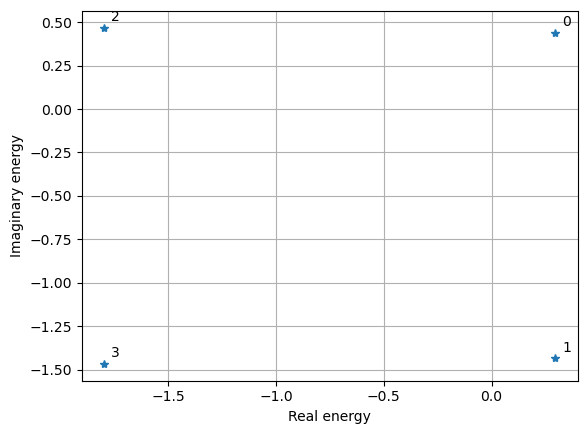
\includegraphics[height=3cm, width=0.5\textwidth]{2NR_coupled_pendula_spectrum.png}
    \end{figure}
    \begin{figure}
        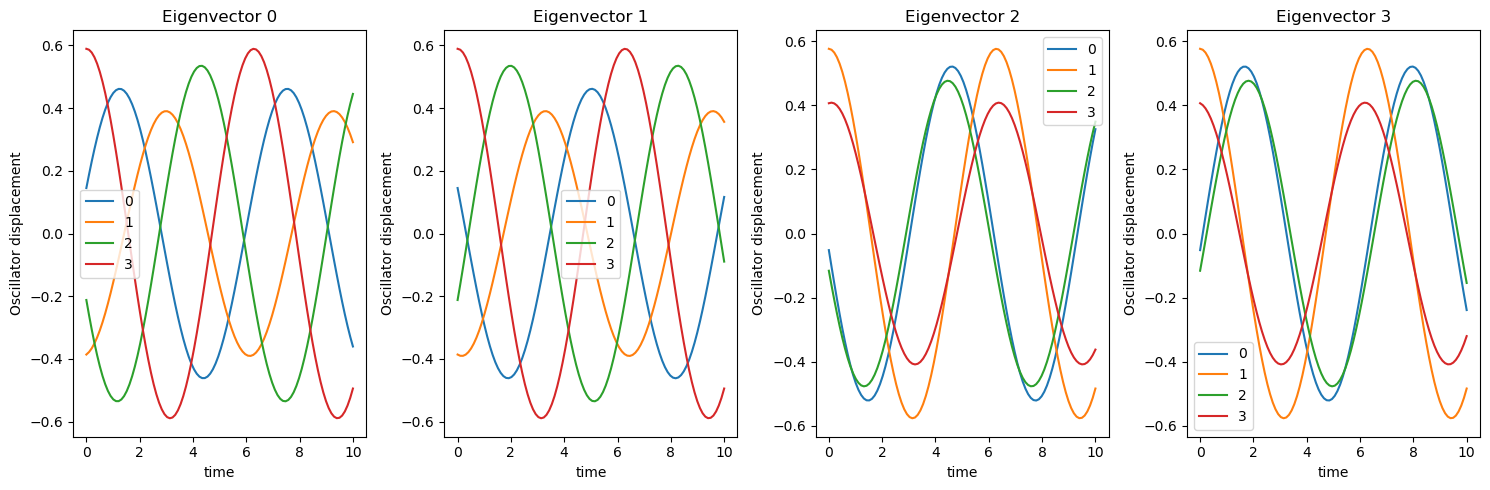
\includegraphics[height=3cm, width=\textwidth]{2NR_coupled_pendula_eigenvectors.png}
    \end{figure}
\end{frame}

\begin{frame}[allowframebreaks]{Lieb lattice of non-reciprocal pendula}
    % We consider a Lieb lattice of non-reciprocal pendula. 
    % \begin{figure}
    %     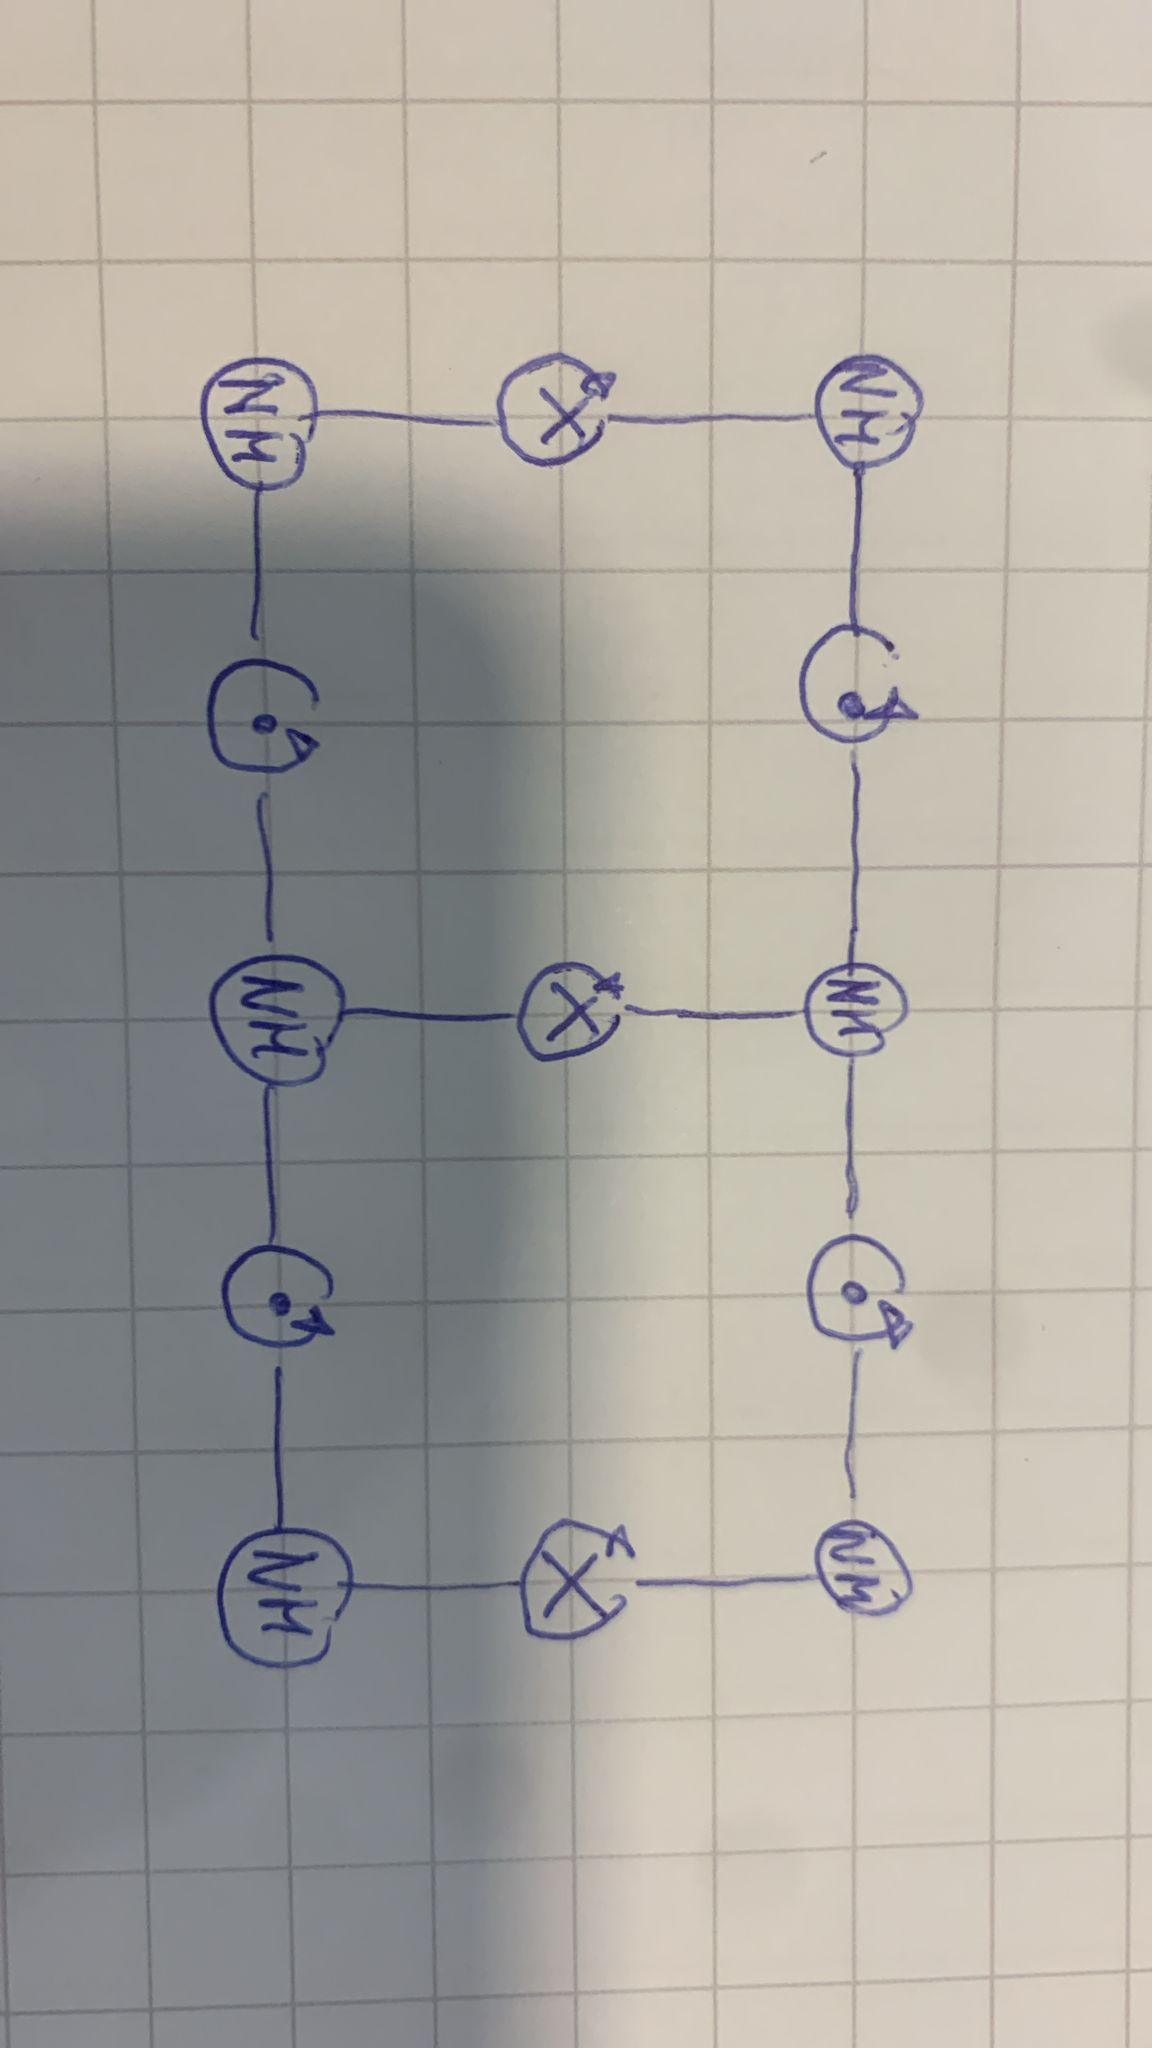
\includegraphics[rotate=90, width = 0.5\textwidth]{WhatsApp Image 2025-10-10 at 12.15.01.jpeg}
    % \end{figure}
    % \framebreak 
    It seems like there are modes with zero energy in certain directions %- the band is flat; but not at E=0, 
    % I guess you can tune that with chemical potential \\
    % Other bands look more nomral with somewhat well shape \\
    Real spectrum:
    \begin{figure}
        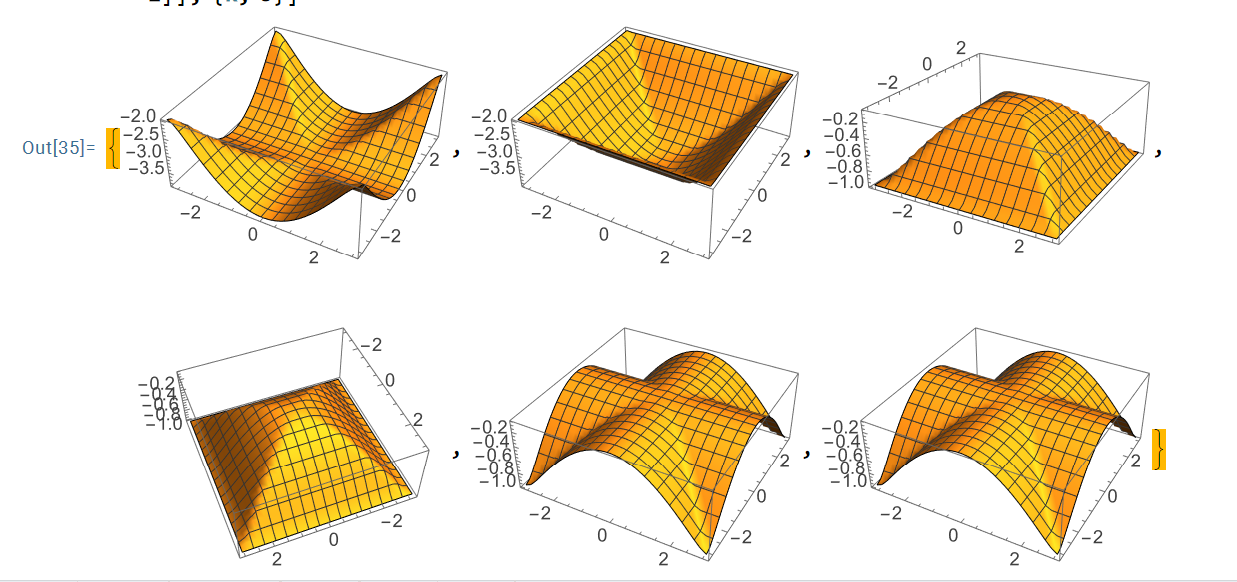
\includegraphics[width = 0.5\textwidth]{non_reciprocal_Lieb_real_energies.png}
    \end{figure}
    %\framebreak 
    Imaginary spectrum:
    \begin{figure}
        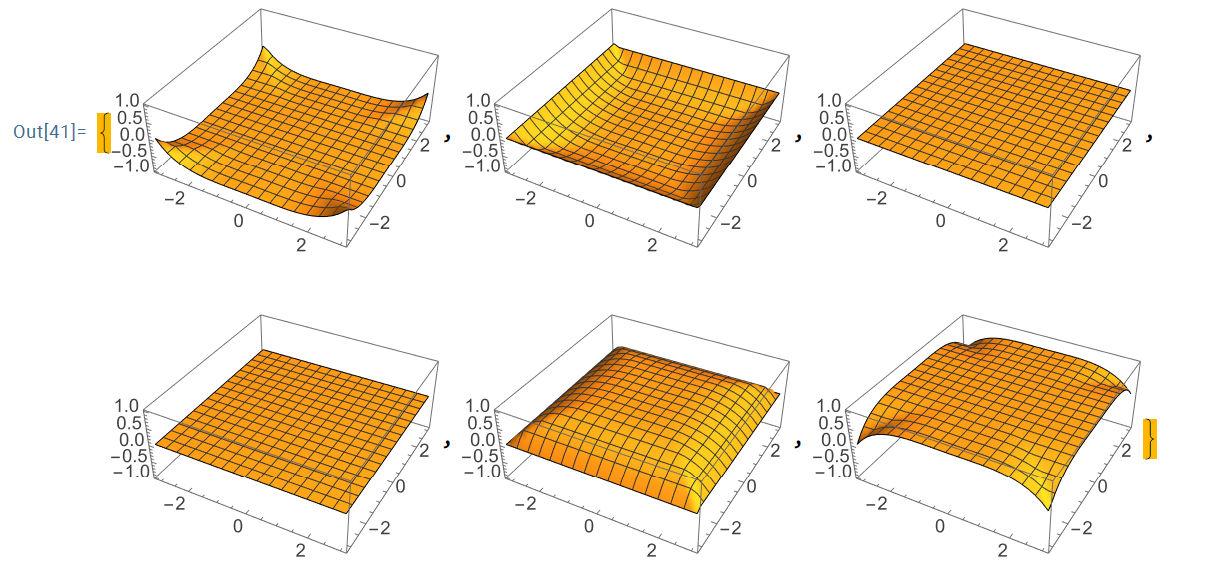
\includegraphics[width = 0.5\textwidth]{non_reciprocal_Lieb_imag_energies.png}
    \end{figure}
\end{frame}

\begin{frame}{Hatano-Nelson ladder PBC}
    \begin{figure}
        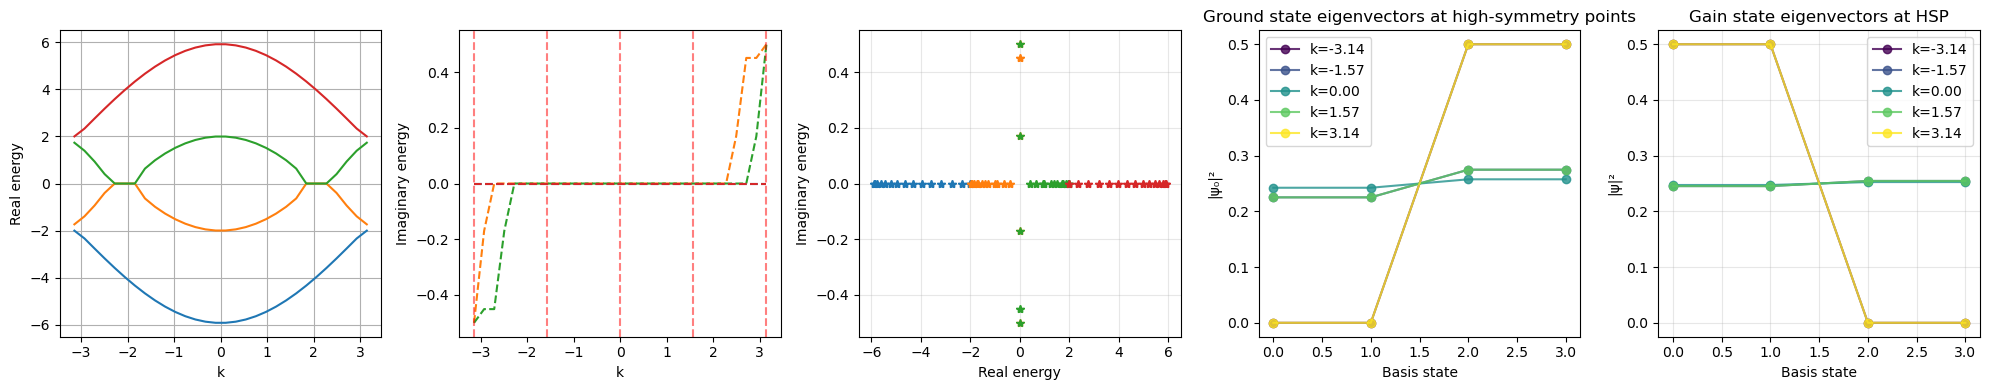
\includegraphics[width=\textwidth]{H-N_ladder_PBC_imaginarypotential.png}
        \caption{Hatano-Nelson ladder PBC with imaginary onsite potential.}
    \end{figure}
    \begin{figure}
        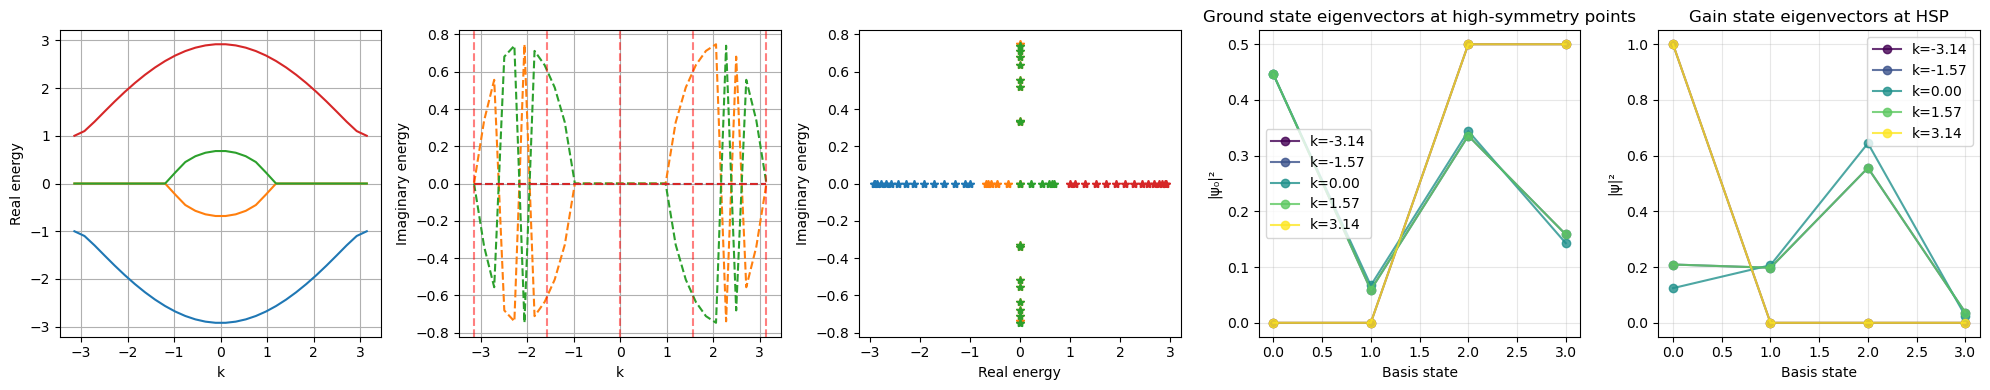
\includegraphics[width=\textwidth]{H-N_ladder_PBC_nonreciprocal.png}
        \caption{Hatano-Nelson ladder PBC with non-reciprocal hopping.}
    \end{figure}
\end{frame}

\begin{frame}[allowframebreaks]{Hatano-Nelson ladder OBC}
    \begin{figure}
        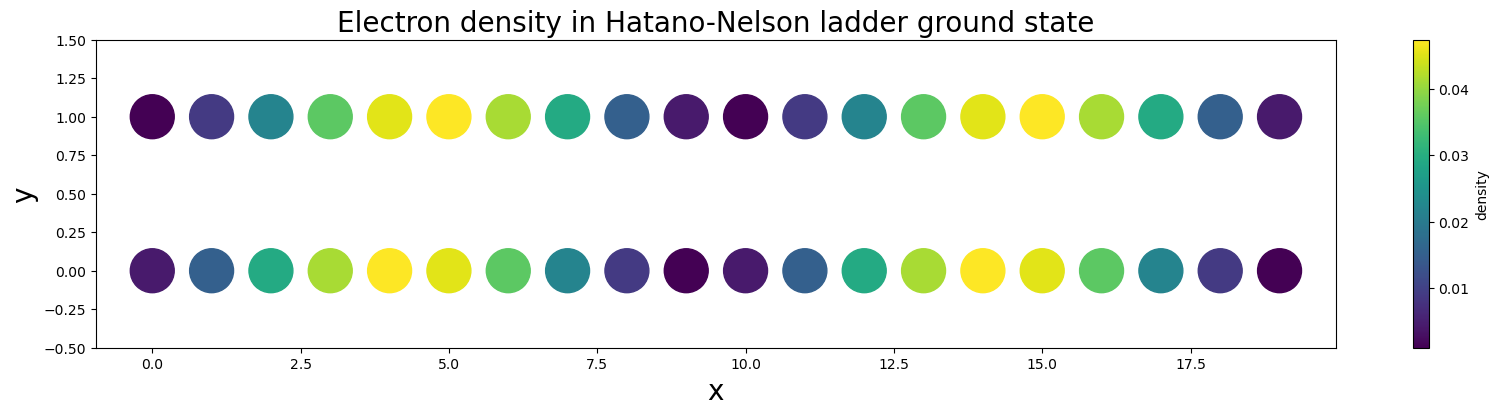
\includegraphics[width=\textwidth]{H-N_ladder_OBC_U=0.png}
        \caption{Hatano-Nelson ladder OBC ordinary: U=0 and reciprocal hopping.}
    \end{figure}
    \framebreak
    \begin{figure}
        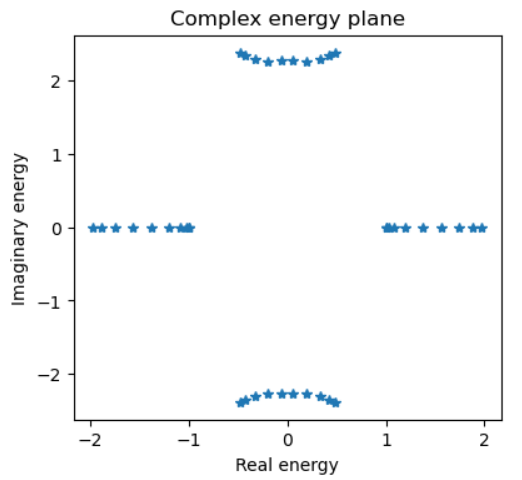
\includegraphics[width=0.5\textwidth]{H-N_ladder_OBC_spectrum_imag_pot.png}
        \caption{Spectrum of Hatano-Nelson ladder OBC with imaginary onsite potential.}
    \end{figure}
    \framebreak
    \begin{figure}
        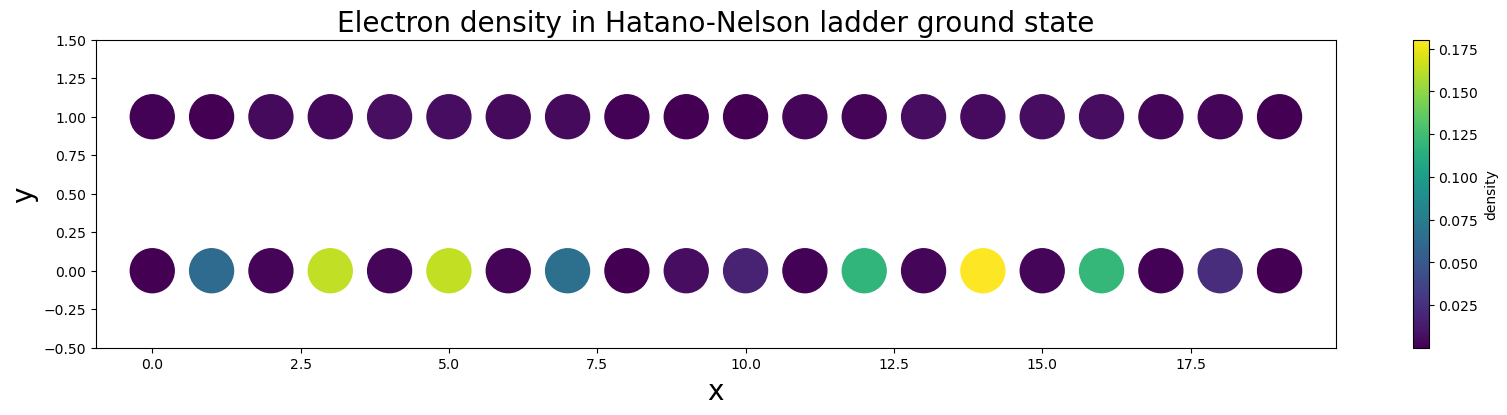
\includegraphics[width=\textwidth]{H-N_ladder_OBC_imag_pot.png}
        \caption{Hatano-Nelson ladder OBC with imaginary onsite potential.}
    \end{figure}
    \framebreak
    \begin{figure}
        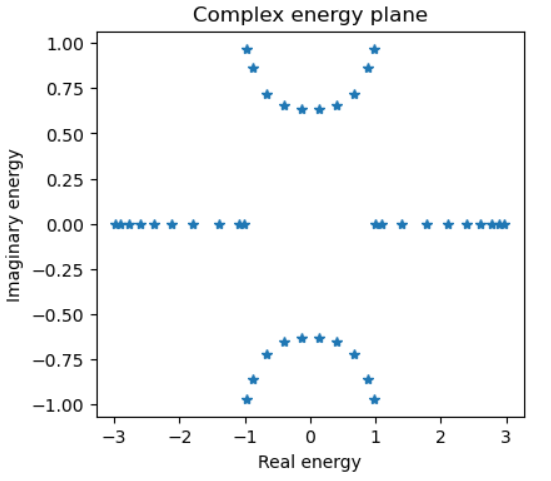
\includegraphics[width=0.5\textwidth]{H-N_ladder_OBC_spectrum_non_rec.png}
        \caption{Spectrum of Hatano-Nelson ladder OBC with non-reciprocal hopping.}
    \end{figure}
    \framebreak
    \begin{figure}
        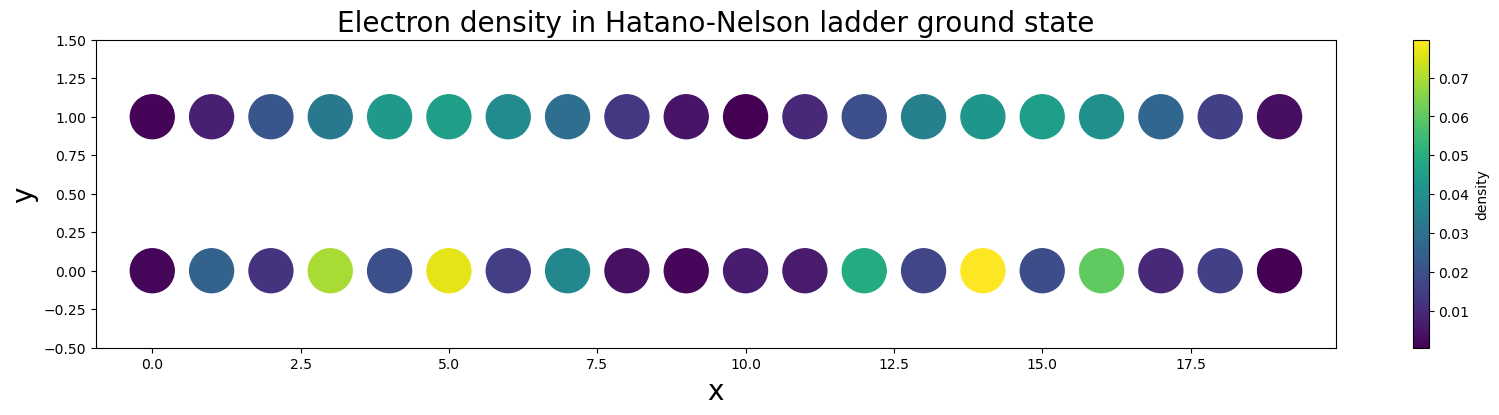
\includegraphics[width=\textwidth]{H-N_ladder_OBC_non_recipr.png}
        \caption{Hatano-Nelson ladder OBC with non-reciprocal hopping.}
    \end{figure}
\end{frame}

\begin{frame}[allowframebreaks]{Ongoing: bilayer Lieb lattice}
    Stack Lieb lattices 
    \begin{figure}
        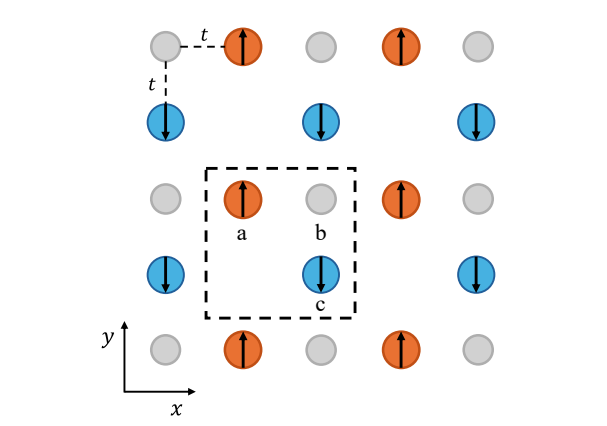
\includegraphics[width=0.5\textwidth]{Lieb_lattice.png}
        \caption{\cite{visser2023}}
    \end{figure}
    \begin{figure}
        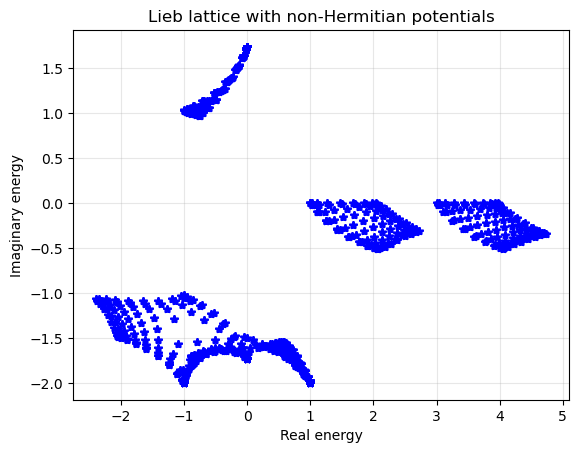
\includegraphics[width=0.5\textwidth]{bilayer_lieb_imaginarypot.png}
        \caption{Spectrum of bilayer Lieb lattice with imaginary onsite potential.}
    \end{figure}
\end{frame}


\section{Summary}

\begin{frame}{Summary}
    \begin{alertblock}{Goal}
        Study altermagnetism and non-hermiticity in classical analogues 
    \end{alertblock}
    \vfill
    \begin{itemize}
        \item Altermagnets: $C_4\mathcal{T}$ symmetry can lead to anisotropic and spin-momentum locking propagation \vfill
        \item Non-hermitian skin effect: waves localized at boundaries \vfill
        \item Classical analogues enable experimental realization
    \end{itemize}
\end{frame}

% \begin{frame}{References}
%     \bibliographystyle{apsrev4-1} % or ieeetr, plain, etc.
%     \bibliography{bibliography}
%     \nocite{*}
% \end{frame}

\section*{Annex}

\begin{frame}[noframenumbering]{Activity}
    The classical analogue of non-hermiticity of Hatano-Nelson is non-reciprocity. \pause
    \vfill
    Activity: internal energy source. \pause 
    \vfill
    There are different ways to achieve activity:  \pause
    \begin{itemize}
        \item Negative damping \pause
        \item Time delay \pause 
        \item \textbf{Non-reciprocity}
    \end{itemize}
\end{frame}

\begin{frame}[noframenumbering]{2 interacting non-reciprocal pendula}
    \begin{figure}
        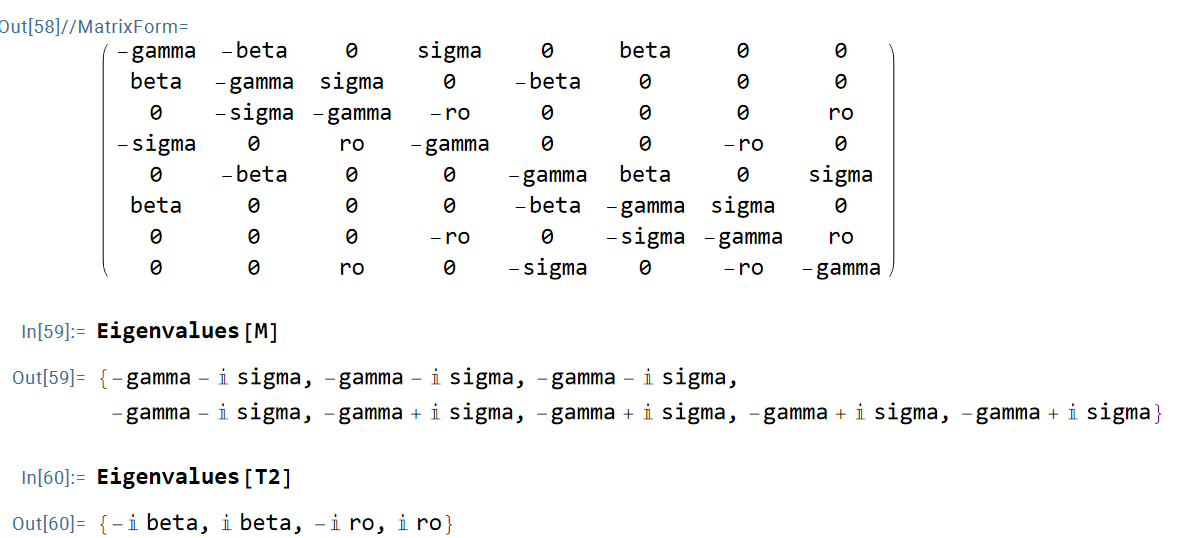
\includegraphics[width = \textwidth]{2NRpendula.png}
    \end{figure}
\end{frame}

\begin{frame}[noframenumbering]{Mechanical altermagnet}
    \begin{itemize}
        \item Focus on anisotropic wave propagation feature of altermagnets
        \item Exp: build on Amber's work: stack 2 toy layers
        \item Th: construct model and explain observations
        \item Study propagation of waves
        \item Main source: Amber's thesis
        %\item Best case scenario: 
        %\item PROS: 
        %\item CONS: 
    \end{itemize}
    \begin{figure}
        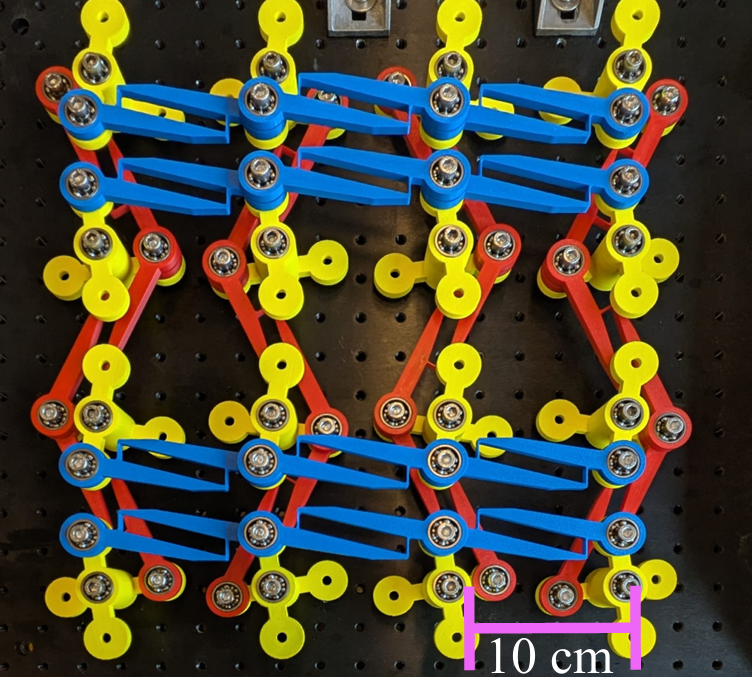
\includegraphics[width=0.5\textwidth]{mechanical_AM_Amber_toy.png}
    \end{figure}
\end{frame}

\begin{frame}[noframenumbering]{Piezoelectric}
    \begin{itemize}
        \item Exp: build altermaterial using capacitors with piezoelectric response
        \item Th: construct microscopic quantum model and compare
        \item Auxetic piezo
        \item Best case scenario: show piezoelectric properties of alterelectrics
        \item Review by Gao, Sharma
    \end{itemize}
    \begin{figure}
        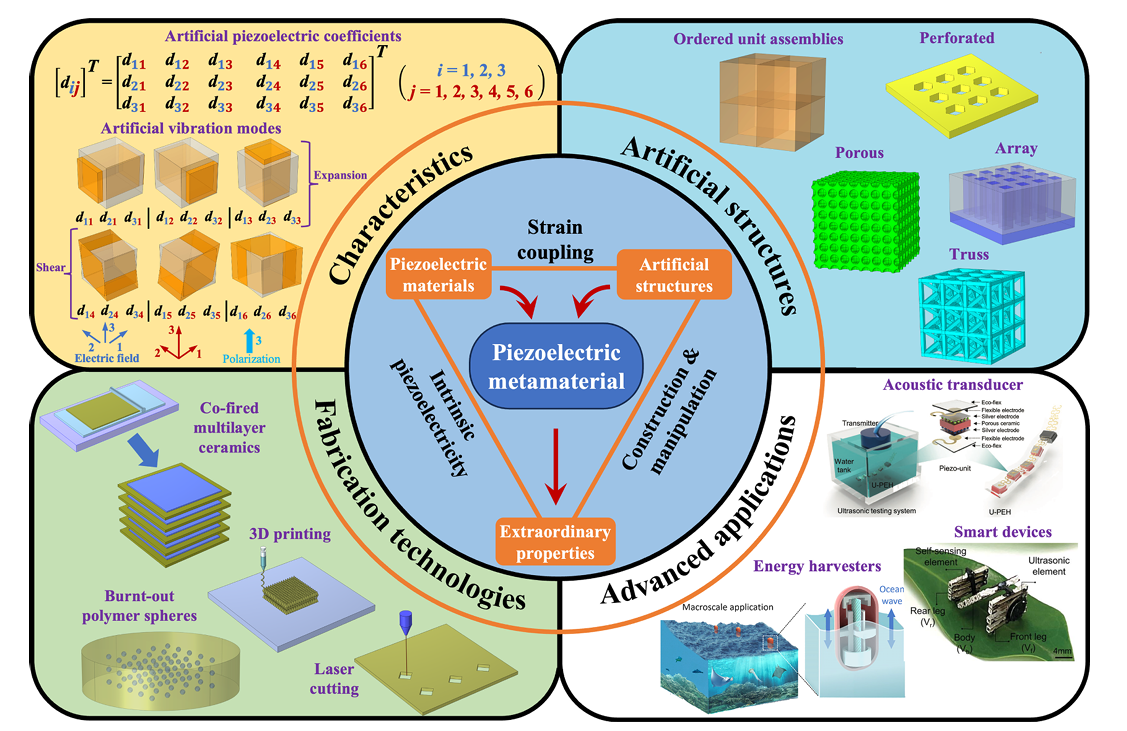
\includegraphics[width=0.5\textwidth]{piezoelectric_metamaterials.png}
    \end{figure}
\end{frame}

\begin{frame}[noframenumbering]{Non-hermiticity}
    \begin{itemize}
        \item Combine altermagnetic symmetry with non-hermiticity
        \item Exp: stack Yuan's cubes with odd elasticity
        \item Study waves propagating
        \item Gain-momentum locking
        \item Th: write analogous quantum hamiltonian and analyse it
    \end{itemize}
     \begin{figure}
        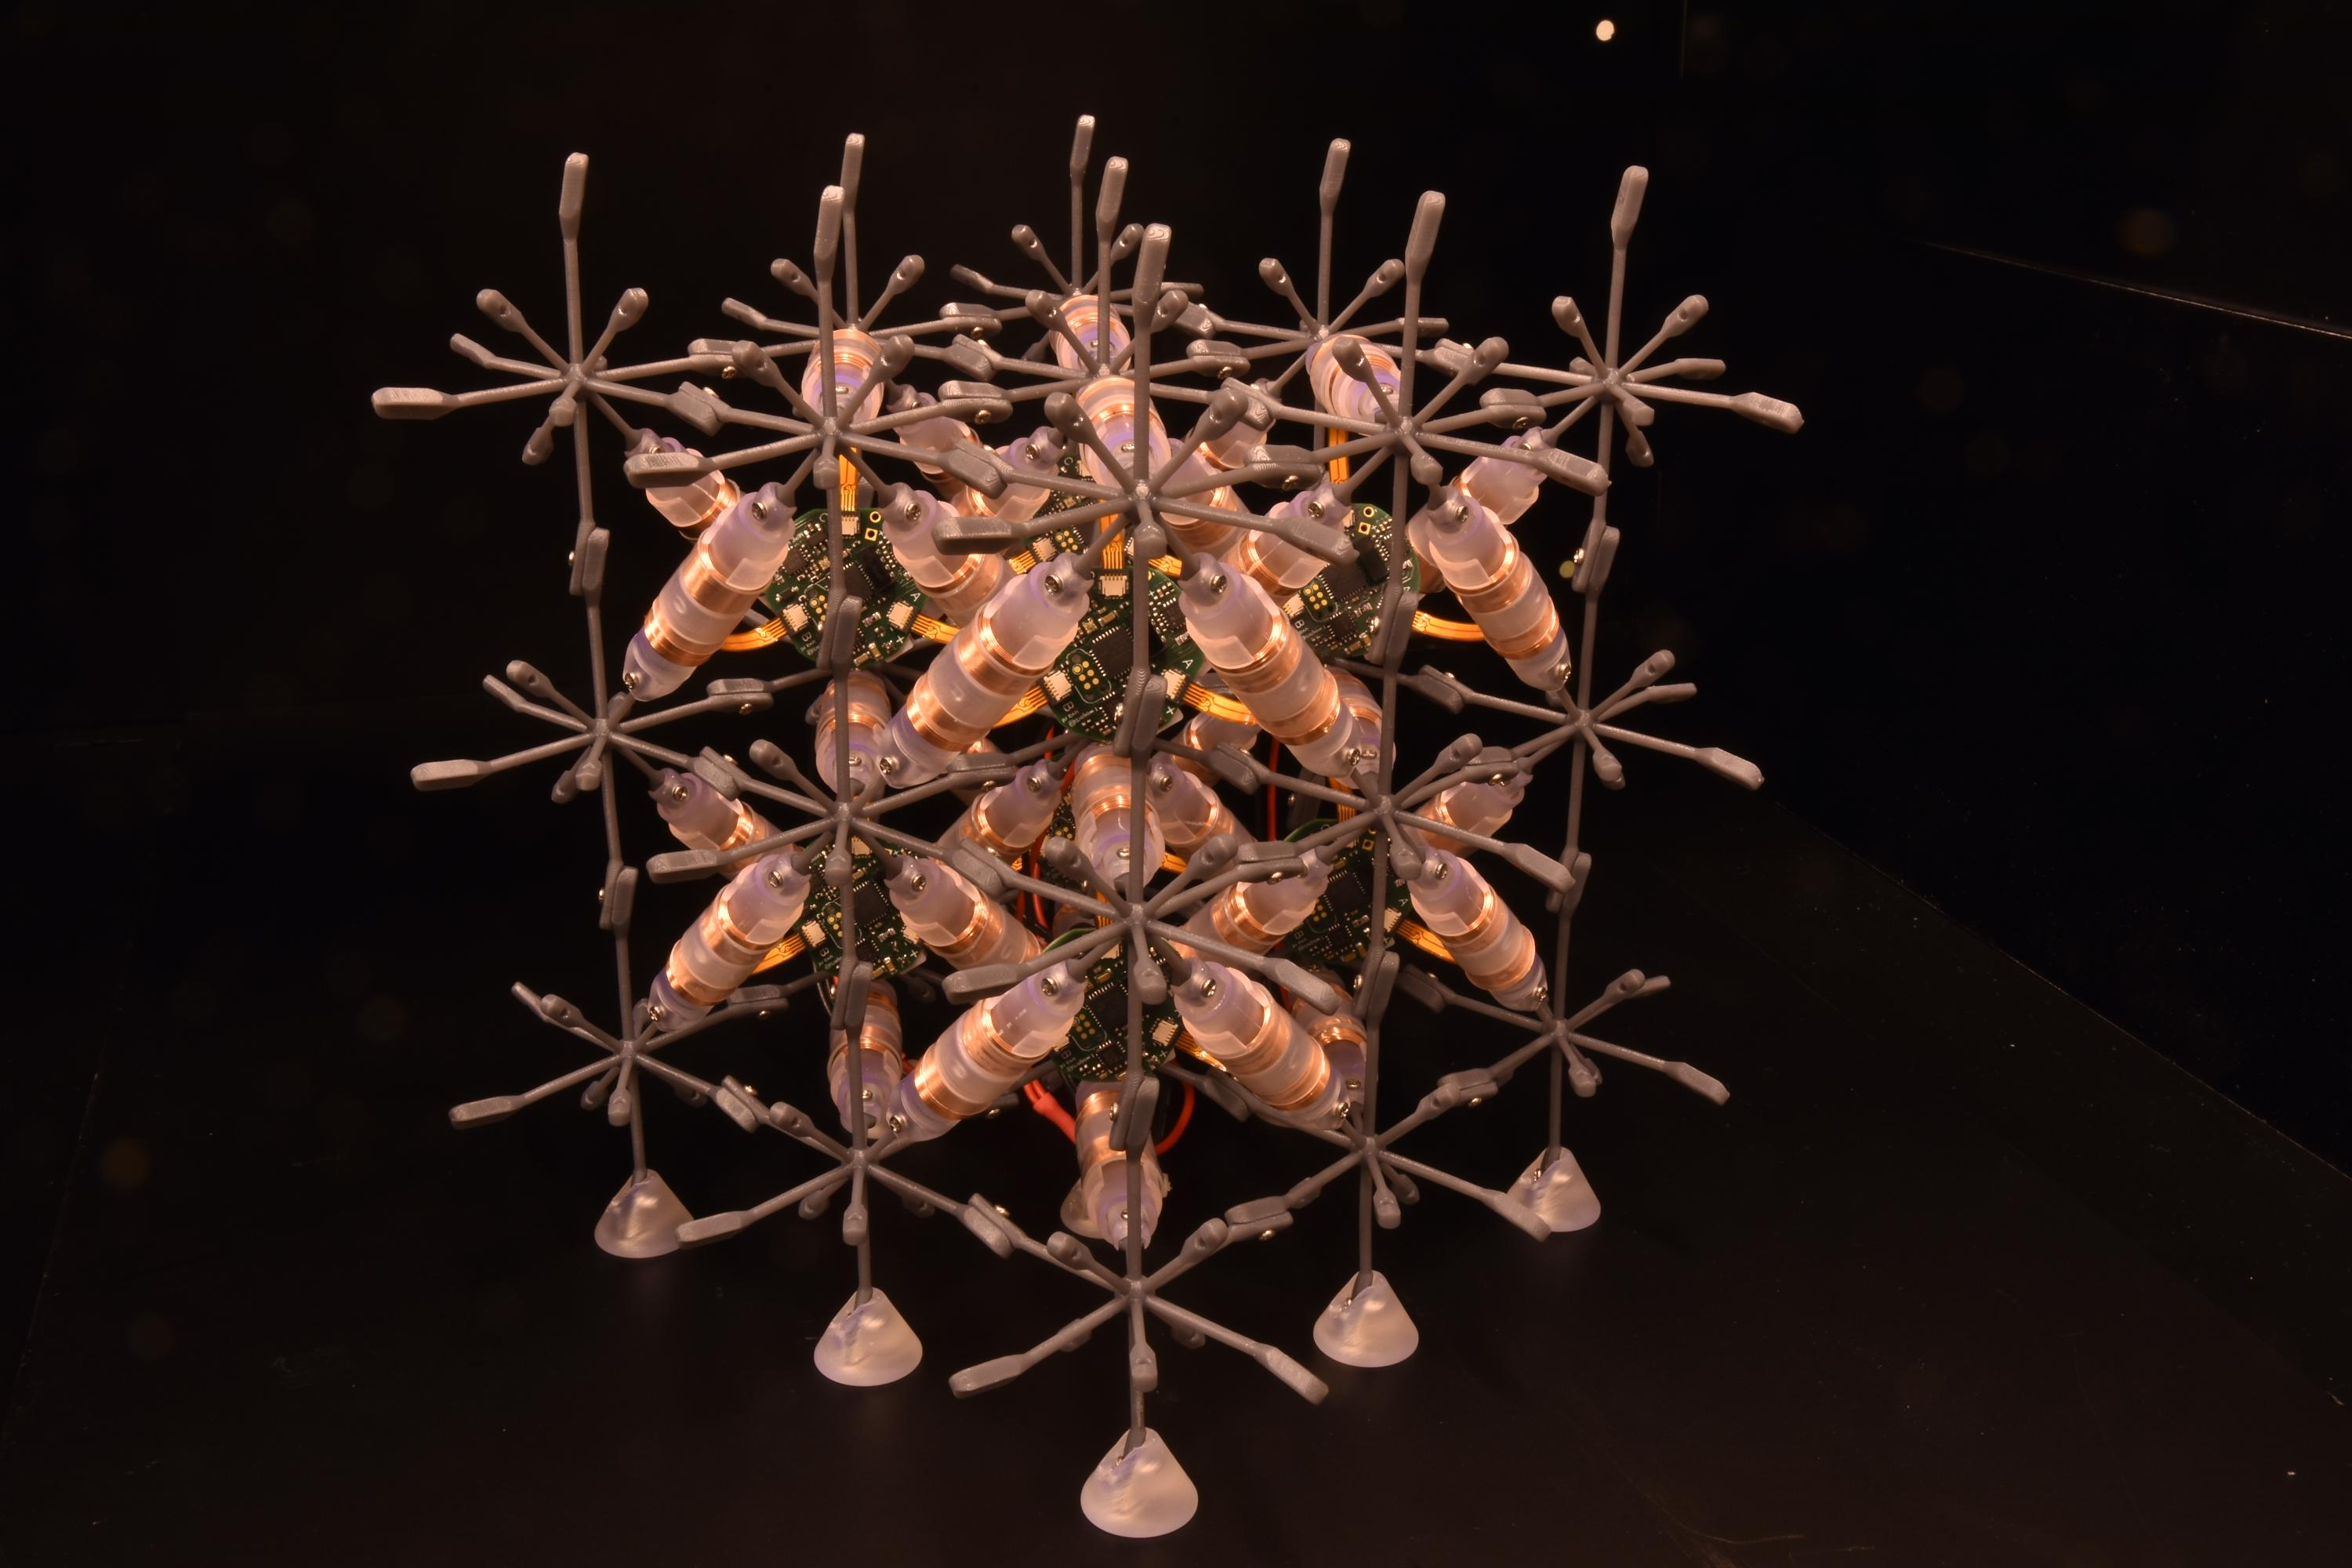
\includegraphics[width=0.5\textwidth]{Yuan_robot.jpeg}
    \end{figure}
\end{frame}

\begin{frame}[noframenumbering]{Other}
    \begin{itemize}
        \item Metamaterials with higher order altermagnet symmetries
        \item Consider other rotations besides 90º
        \item For theory in general: band structure, ground state, excitations, topological properties, defects
    \end{itemize}
\end{frame}

\begin{frame}[noframenumbering]{Research plan}
    \begin{itemize}
        \item Calculate band structure of mechanical Lieb lattice
        \item Simulate Lieb lattice of non-reciprocal units
        \item Build Lieb lattice of non-reciprocal units
    \end{itemize}
    Possible questions
    \begin{itemize}
        \item Are there skin effects?
    \end{itemize}
\end{frame}

\begin{frame}[noframenumbering]{Do altermagnets always have hyperbolic dispersion?}
    \pause
    \begin{enumerate}
        \item Break TRS \pause
        \item C4T symmetry \pause
        \item Inversion symmetry \pause
        \item Zero magnetisation
    \end{enumerate}
\end{frame}

\begin{frame}[noframenumbering]{Hatano-Nelson ladder}
    Parameters: U = 1, r = 2, t = 1, a = 1
    \begin{figure}
        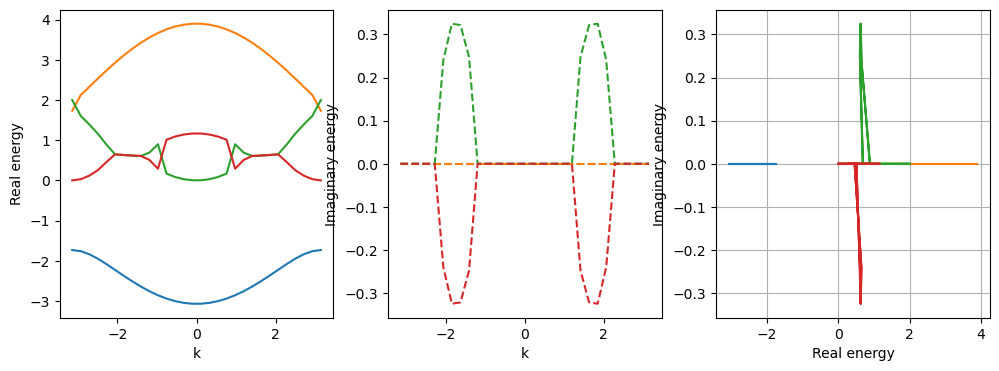
\includegraphics[width=\textwidth]{hatano_ladder_spectrum.png}
    \end{figure}
    \begin{figure}
        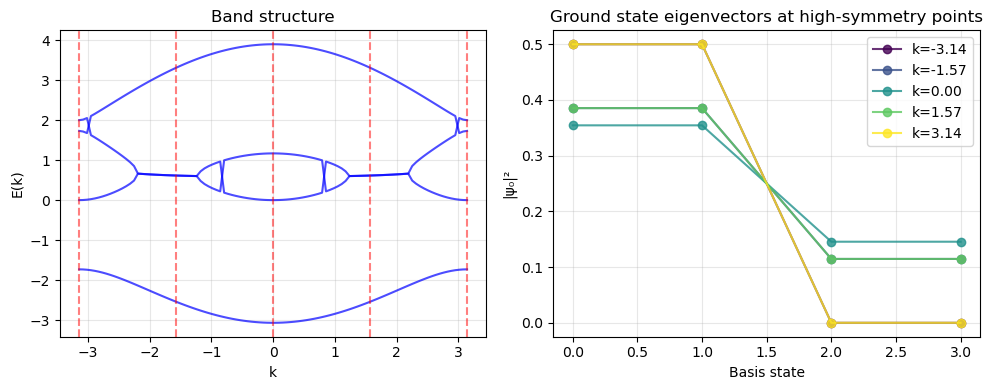
\includegraphics[width=0.5\textwidth]{hatano_ladder_eigenstates.png}
    \end{figure}
\end{frame}

\begin{frame}[noframenumbering]
\begin{figure}
    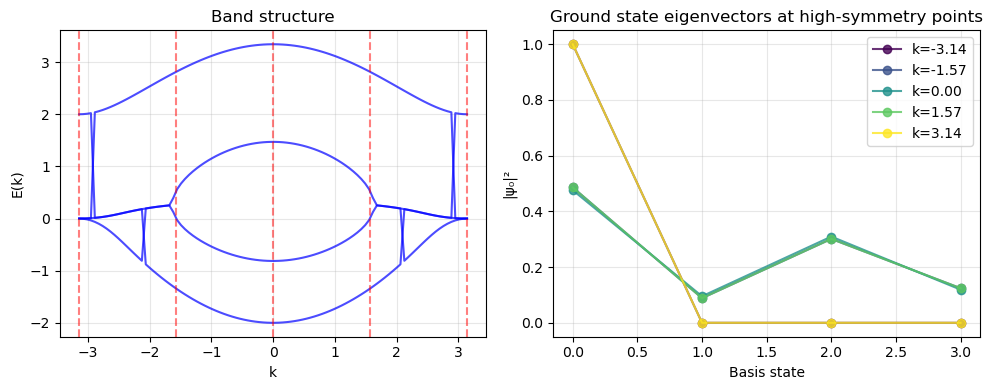
\includegraphics[width=\textwidth]{hatano_ladder_asymmetric.png}
\end{figure}
\end{frame}

\end{document}